%%%%%%%%%%%%%%%%%%%%%%%%%%%%%%%%%%%%%%%%%
% Large Colored Title Article
% LaTeX Template
% Version 1.1 (25/11/12)
%
% This template has been downloaded from:
% http://www.LaTeXTemplates.com
%
% Original author:
% Frits Wenneker (http://www.howtotex.com)
%
% License:
% CC BY-NC-SA 3.0 (http://creativecommons.org/licenses/by-nc-sa/3.0/)
%
%%%%%%%%%%%%%%%%%%%%%%%%%%%%%%%%%%%%%%%%%

%----------------------------------------------------------------------------------------
%	PACKAGES AND OTHER DOCUMENT CONFIGURATIONS
%----------------------------------------------------------------------------------------

\documentclass[DIV=calc, paper=letter, fontsize=12pt]{scrartcl}	 % A4 paper and 11pt font size

\usepackage{lipsum} % Used for inserting dummy 'Lorem ipsum' text into the template
\usepackage[english]{babel} % English language/hyphenation
\usepackage[protrusion=true,expansion=true]{microtype} % Better typography
\usepackage{amsmath,amsfonts,amsthm} % Math packages
\usepackage[svgnames]{xcolor} % Enabling colors by their 'svgnames'
\usepackage[hang, small,labelfont=bf,up,textfont=it,up]{caption} % Custom captions under/above floats in tables or figures
\usepackage{booktabs} % Horizontal rules in tables
\usepackage{fix-cm}	 % Custom font sizes - used for the initial letter in the document

\usepackage{sectsty} % Enables custom section titles
\allsectionsfont{\usefont{OT1}{phv}{b}{n}} % Change the font of all section commands

\usepackage{fancyhdr} % Needed to define custom headers/footers
\pagestyle{fancy} % Enables the custom headers/footers
%\usepackage{lastpage} % Used to determine the number of pages in the document (for "Page X of Total")
\usepackage{url} % Used to properly format URLs
\usepackage{epigraph} % Used to format epigraphs
%\usepackage{listings} %Used to highlight python code in appendix
\usepackage{multicol}
\usepackage{fullpage}
\usepackage[procnames]{listings}
\usepackage{color}
\usepackage{minted}
\newminted{python}{fontsize=\footnotesize}
\usepackage{graphicx}

% Headers - all currently empty
\lhead{}
\chead{}
\rhead{}

% Footers
\lfoot{}
\cfoot{}
\rfoot{}
%\rfoot{\footnotesize Page \thepage\ of \pageref{LastPage}} % "Page 1 of 2"

\renewcommand{\headrulewidth}{0.0pt} % No header rule
\renewcommand{\footrulewidth}{0.4pt} % Thin footer rule

\usepackage{lettrine} % Package to accentuate the first letter of the text
\newcommand{\initial}[1]{ % Defines the command and style for the first letter
\lettrine[lines=3,lhang=0.3,nindent=0em]{
\color{DarkGoldenrod}
{\textsf{#1}}}{}}

%----------------------------------------------------------------------------------------
%	TITLE SECTION
%----------------------------------------------------------------------------------------

\usepackage{titling} % Allows custom title configuration

\newcommand{\HorRule}{\color{DarkGoldenrod} \rule{\linewidth}{1pt}} % Defines the gold horizontal rule around the title

\pretitle{\vspace{-30pt} \begin{flushleft} \HorRule \fontsize{40}{40} \usefont{OT1}{phv}{b}{n} \color{DarkRed} \selectfont} % Horizontal rule before the title

\title{Preposition Stranding in Printed English} % Your article title

\posttitle{\par\end{flushleft}\vskip 0.5em} % Whitespace under the title

\preauthor{\begin{flushleft}\large \lineskip 0.5em \usefont{OT1}{phv}{b}{sl} \color{DarkRed}} % Author font configuration

\author{Walker Davis, } % Your name

\postauthor{\footnotesize \usefont{OT1}{phv}{m}{sl} \color{Black} % Configuration for the institution name
Princeton University % Your institution

\par\end{flushleft}\HorRule} % Horizontal rule after the title

\date{} % Add a date here if you would like one to appear underneath the title block

%----------------------------------------------------------------------------------------

%----------------------------------------------------------------------------------------

\begin{document}

	\definecolor{keywords}{RGB}{255,0,90}
	\definecolor{comments}{RGB}{0,0,113}
	\definecolor{red}{RGB}{160,0,0}
	\definecolor{green}{RGB}{0,150,0}
	 
	\lstset{language=Python, 
	        basicstyle=\ttfamily\small, 
	        keywordstyle=\color{keywords},
	        commentstyle=\color{comments},
	        stringstyle=\color{red},
	        showstringspaces=false,
	        identifierstyle=\color{green},
	        procnamekeys={def,class}}

\maketitle % Insert title

%\thispagestyle{fancy} % All pages have headers and footers

%----------------------------------------------------------------------------------------
%	ABSTRACT
%----------------------------------------------------------------------------------------
\begin{multicols}{2} % Two-column layout throughout the main article text

\section{Abstract}

\noindent The grammatical rule against preposition stranding, or the act of ending a sentence with a preposition, began as a stylistic convention popularized by British poet and author John Dryden in 1672. Dryden's writing about the issue mentioned that he noticed the tendency to end sentences with prepositions in the writing of many recent authors, such as William Shakespeare. Using a combination of Python scripts, SQLite databases, and text files downloaded from Project Gutenberg, the frequency of preposition stranding over the history of written English was examined. It was found that there was a noticeable spike in the absolute and relative frequency of stranded prepositions in the first half of the 17th century, which then dropped dramatically in the latter half of the 1600s. The frequency of preposition stranding then increased steadily over the years until the present day. While it is unclear how much influence John Dryden held over the decrease in stranding in the late 1600s, the data at least suggests that Dryden was motivated by a sharp increase in stranding over his lifetime. Additionally, it was found that strongly locative prepositions are more frequently found at the end of a sentence as proportion.

%----------------------------------------------------------------------------------------
%	ARTICLE CONTENTS
%----------------------------------------------------------------------------------------


\section{Introduction}

\epigraph{This is the sort of bloody nonsense up with which I will not put!}{Winston Churchill (apocryphal)}

Preposition stranding is a perennial favorite subject for strict grammar teachers and those who 
fashion themselves to be the standard bearers of ``proper'' English. However, what is often taught
in school as an immutable grammatical rule can often result in slightly absurd sentences, as seen
in the included Churchill epigraph. The (apocryphal) story behind the quote is that an overzealous 
aide to Churchill edited one of his speeches so that none of his sentences ended with a preposition,
but Churchill found the alterations to be so stylistically abhorrent he decided to reprimand the 
well-meaning individual with his own grammatical convention\cite{Churchill}. 

The prohibition on preposition stranding can most likely trace its
origins to the 17th century writer John Dryden. Dryden was an English writer, playwright, and critic
who was a central literary force in Restoration England. His works included \emph{Conquest of Granada}, \emph{All for Love}, and a translated version of the Aeneid. Dryden wrote in the ``Defense of the Epilogue'' of the \emph{Conquest of Granada} that ``[He] cast [his] eyes but by chance on \emph{Catiline}\footnote{\emph{Catiline} is a play by Ben Jonson about tragedy of the Roman politician Catiline.}; and in the first three or four pages, found enough to see that Jonson writ not correctly'' \cite{Defense}. The line that Dryden specifically cited later in the essay was ``The waves and dens of beasts could not receive \ The bodies those souls were frighted \emph{from}''. Dryden expressed displeasure at having a preposition end a sentence, but he did not further describe why he disliked it. Later, grammarian Robert Lowth wrote in his 1762 book \emph{A Short Introduction to English Grammar} that ``This is an Idiom which our language is strongly inclined to; it prevails in common conversation, and suits very well with the familiar style in writing; but the placing of the Preposition before the Relative is more graceful, as well as more perspicuous; and agrees much better with the solemn and elevated Style,'' and drew ties to Latin's prohibition against ending sentences with prepositions \cite{Lowth}.

The motivation for this project is to examine how grammatical conventions can become 
grammatical rules. It remains unclear if the preposition stranding that Dryden complained about
was a prevalent feature of the language beforehand, or if it was restricted to the few instances he specifically noted in the writing of William Shakespeare and Ben Jonson; it is also unknown how quickly or effectively the convention was adopted. Further, investigating which prepositions are most frequently used at the end of a sentence could lend additional insight into preposition stranding. 

%------------------------------------------------

\section{Methods}

In order to track the usage of prepositions in the English language, I searched a large corpus and 
logged the appearance of prepositions and the occurences of stranded prepositions.
To do this, the entire catalog of Project Gutenberg, a freely available repository of books in the
public domain, was downloaded to form a corpus of approximately 40,000 books.

To log the usage of prepositions, a Python script and a SQLite\footnote{SQL: Structured Query Language} database were used. The Python script implemented a simple regular expression, a tool used in
computer science for substring matching, which is the core of the research problem posed by searching
through the Gutenberg corpus. Regular expressions are essentially enhanced search queries
that can search for matching characters in a set, repetitions of a series of characters, and
even branching logic (eg. either ABC \emph{or} CBA). For illustrations' sake, the regular expression used for 
finding stranded prepositions was: 
\begin{equation*}\text{(aboard $\vert$ above $\vert$ about $\vert$ etc.)[.;?!]}\end{equation*} The ``pipe'' symbol ($\vert$),
denotes a logical exclusive or, which means that exactly one of the words present in the section enclosed by
parentheses (i.e. one preposition) must be included in a substring for it to be valid. The block of punctuation marks 
concatenated with the parenthetical section makes it so that a valid substring must be composed of
one of the approved prepositions and one character from the set of punctuation marks. 
Commas and quotation marks were chosen to not be considered
punctuation because their use is largely based upon an author's usage convention and would register several
false positives. Additionally, I elected to \emph{not} attempt to employ various natural language processing
techniques to the samples. Properly parsing the sentence into parts of speech and clauses would 
allow several false negatives to be counted, but it would be more computationally difficult than simply searching with regular expressions and due to the inherent inaccuracy of parsing, would 
result in false positives being reported. With a corpus in the realm of hundreds of millions of words, 
the 94\% to 99\% accuracy of modern open source natural language processing tools would result
in a large amount of variance solely due to the behavior of the parser. These reasons combined lead
to my decision to focus only on prepositions immediately followed by punctuation, since the results
would not be affected by technical issues.

Whenever a preposition or a stranded preposition were found, relevant fields in SQLite database were updated. Once the corpus was processed, MATLAB was used to generate summary statistics total amount of prepositions and the amount of stranded prepositions for 
each time interval, as well as  charts and figures.   
%------------------------------------------------

\section{Results}

\subsection{Preposition Stranding}

\begin{table*}[t]
  \centering
   \caption{Data collected normalized to a corpus size of 1000000 words for each time bin.}
  %\begin{tabular}{ | l | l | l | p{5cm} |}
  \begin{tabular}{| l | l | l | p{3cm} | p{3cm} |}
    \hline

   	 \multicolumn{1}{|p{2cm}|}{\centering Time \\ Period} & \multicolumn{1}{|p{2.5cm}|}{\centering Stranded \\ Prepositions} &  \multicolumn{1}{|p{2.5cm}|}{\centering Total \\ Prepositions} &  \multicolumn{1}{|p{2.9cm}|}{\centering Stranded / Total \\ Prepositions (\%)} &  \multicolumn{1}{|p{3.5cm}|}{\centering Stranded / Total \\ Words (\%)} \\ \hline 
1500-1549 &	622.615 & 	180997.192	& 0.344 & 0.0623 \\ \hline 
1550-1599 	& 605.864	 & 157824.749	 & 0.384	 & 0.0606 \\ \hline 
1600-1649	&1249.283	 & 107492.283	& 1.162 &	0.125 \\ \hline 
1650-1699	& 918.783 &	166400.388	& 0.552 &	0.0919 \\ \hline 
1700-1749	& 1202.342	 & 196187.808	 & 0.613 &	0.120\\ \hline 
1750-1799	& 1085.268	 & 185469.226	& 0.585	 & 0.109 \\ \hline 
1800-1849	& 1549.205	 & 180867.064	& 0.856	 & 0.155 \\ \hline 
1850-1899	& 1968.863	 & 185305.948	& 1.062 &	0.197 \\ \hline 
1900-1949	& 2371.967	 & 171923.209	& 1.380	 & 0.237 \\ \hline 
1950-1999	& 2362.547	 & 155582.675	& 1.519	& 0.236 \\ \hline 

	\end{tabular}
  \label{tab:1}
\end{table*}

\begin{figure*}
	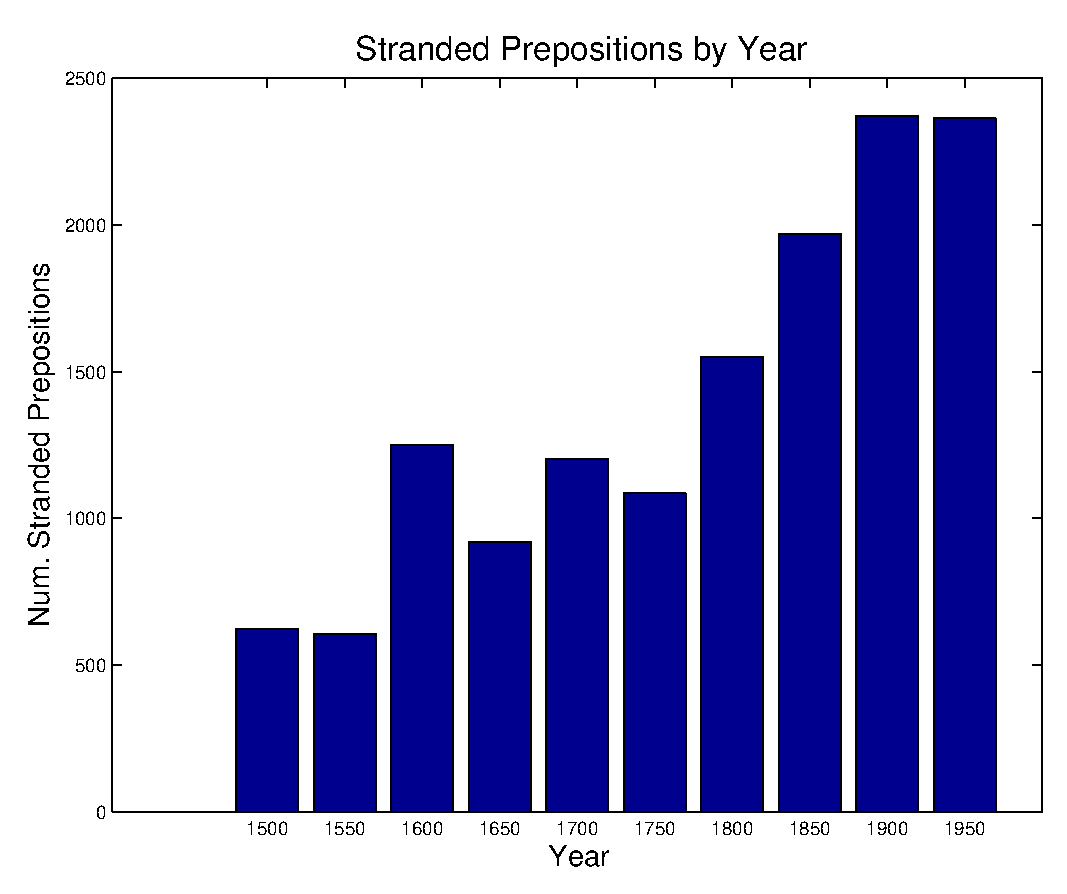
\includegraphics[width=80mm]{preposition1.eps} 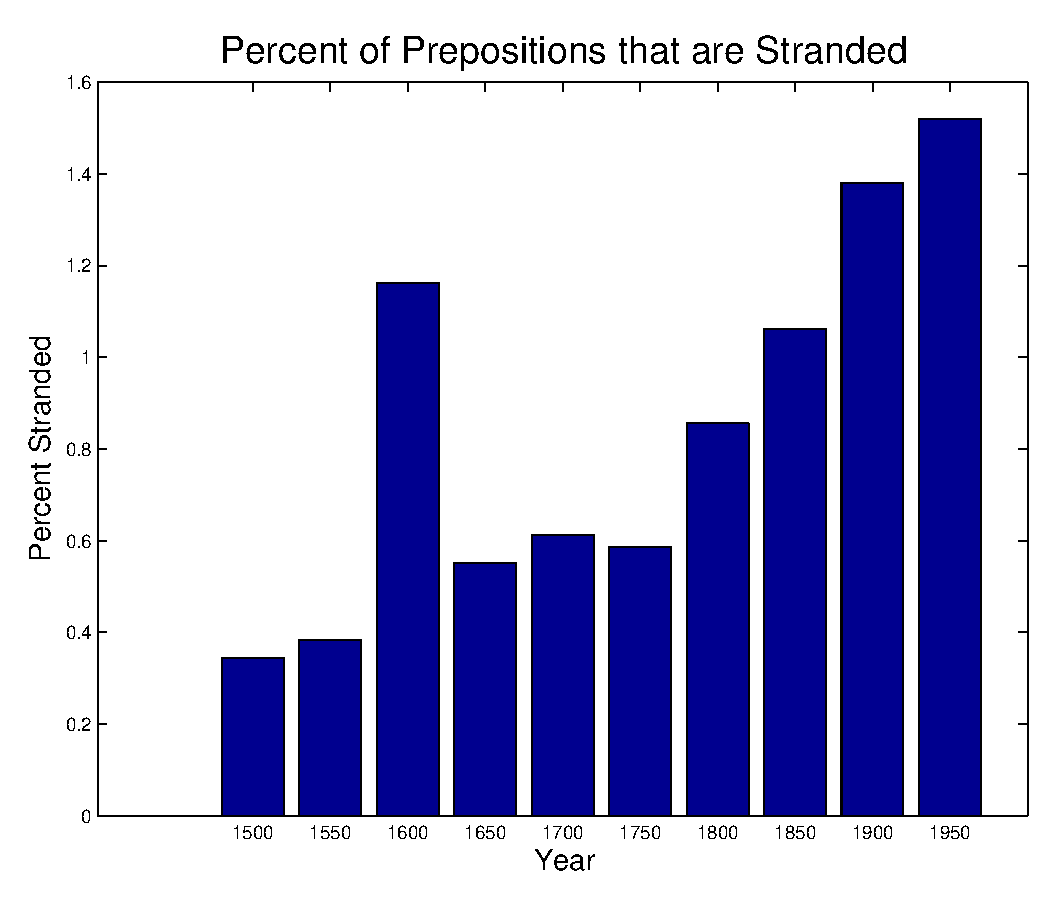
\includegraphics[width=80mm]{preposition2.eps}
	\caption{Left: Absolute occurrences of stranded prepositions by time period. \\Right: Percentage of all prepositions that are stranded by time period.}
\end{figure*}

The results found in Table 1 indicate that preposition stranding occurred at a rate of approximately 600 stranded prepositions per one million words in 16th century writing. This rate jumped to 1250 stranded prepositions per million words in the first half of the 17th century, and then dropped by over a third in the latter half of the century. Preposition stranding then slowly increased to an average of 1143 stranded prepositions per million words in the 1700s. The first half of the 19th century saw a 35\% increase to 1550 stranded prepositions per million words, and then there was another increase of 25\% moving into the late 1800s. The 1900s made a jump to 2360 stranded prepositions per million, remaining relatively constant through the century. These trends are more visually apparent in Figure 1.

Additionally, the ratio of stranded prepositions to total prepositions and stranded prepositions both decreased from 1600-49 to 1650-99 and then resumed a steady climb to 1.519\% and 0.236\% respectively.

\subsection{Preposition Frequency}

%TODODODODODODODODODODODO
\begin{table*}[t]
  \centering
   \caption{Left: The ten most commonly stranded prepositions. \\Right: The ten most commonly used prepositions}
  \begin{tabular}{c | c }
    Preposition & Instances \\ \hline
    up & 1426 \\
    on & 1338 \\
    before & 1116 \\
    in & 1099 \\
    to & 854 \\
    down & 825 \\
    of & 812 \\
    off & 773 \\
    for & 604 \\
    over & 501\\
  \end{tabular}
    \begin{tabular}{c | c }
    Preposition & Instances \\ \hline
    	of	& 311858 \\
to	& 302590\\
in	& 224878\\
for	& 92001\\
on	& 91468\\
as	& 89155\\
with	& 86313\\
at	& 56465\\
by	& 49036\\
but	& 45194\\
    
  \end{tabular}

\end{table*}


The ten most commonly stranded prepositions over the entire corpus of 10235101 words, and the most commonly used prepositions overall are found in Table 2\footnote{Found on page 6; LaTeX does weird things to figures in multi-column documents.}
On, in, to, of, and for are found in both groups. Up, before, down, off, and over are unique to the stranded group. As, with, at, by, and but are all only found in the overall usage group, and all five are 
in the bottom five in terms of usage. 

%------------------------------------------------

\section{Discussion}

\subsection{Preposition Stranding}

While the information found in Figure 1 could lead a reader to believe that Dryden singlehandedly stemmed the flood of stranded prepositions that threatened the English-writing world in the early 17th century, it is unclear how involved he was in the immediate decrease in the latter half of the century. The works surveyed in the first half of the 1600s included a large amount of plays, which were more common in Project Gutenberg's archive for that time period. Since plays are mostly dialouge and stage directions, their structure could lend themselves to having higher amounts of preposition stranding. In a short test, I found that while Shakespeare used a smaller amount of prepositions in his work ($\approx$7\% vs $\approx$11-13\% in prose), he had a very high stranding rate for those prepositions ($\approx$1.75\%). Since plays focus on realistic dialogue, where preposition stranding is often the more natural way of speaking, and stage directions, which are typically terse and focus on describing physical and temporal relations between things, it is possible that the increase of preposition stranding in the early 1600s speaks more to the success of plays in England at the time. The subsequent decrease could also suggest that more prose was preserved from the latter half of the 17th century than plays.
Nonetheless, this data reveals an important fact: preposition stranding \emph{was} on the rise during the time of John Dryden. While John Dryden may be characterized as a ``17th century Latin-obsessed introvert'' in the modern day \cite{SMBC}, it is clear now that he saw a growing stylistic trend that he disagreed with in his era, which led to him creating his style rule; he did not simply think up the style rule after seeing a few isolated examples of preposition stranding, as some may believe. Further, Robert Lowth's 1762 \emph{A Short Introduction to English Grammar} does not appear to have much long-term effect on addressing the stranding dispute, based on the increase from the 1700s to the 1800s.

\subsection{Preposition Frequency}

The way that the most commonly used prepositions and the most commonly stranded prepositions overlap is very interesting. The common elements of the two sets are the top 5 most used prepositions\footnote{of, to, in, for, and on (in that order)}. This suggests that those elements are present in the
most stranded set mostly because of how frequently they are used. %ADD TABLE
The unique elements in the most commonly stranded set are elements that are stranded a disproportionate amount of the time. These are all explicitly locative\footnote{The top ten most frequently stranded prepositions by percentage are below(26.97\%), aboard(22.31\%), inside(15.84\%), outside(15.05\%), before(10.19\%), around(9.17\%), underneath(8.92\%), past(8.59\%), within(8.41\%), and down(7.98\%).}, which suggests that prepositions that deal with physical relationships between the locations of two objects are uniquely predisposed towards being used at the end of a sentence. Preposition stranding predominantly occurs in cases of Wh-questions, pseudo-passives, and relative clauses, all of which typically denote a location. 

\subsection{Sources of Bias}
The samples are inherently biased based on the tendencies of the authors. However, in an attempt to create roughly comparable corpuses for each time period (about a million words each), certain authors can gain a larger amount of influence, given that all of the books are not the same size. Additionally, since Project Gutenberg does not include the original publication date of the books in the  text files that they distribute, it was impossible to completely automate the process. Since I had to manually enter the files to be processed, the corpus was smaller than it could have been under ideal circumstances. This could possibly introduce some systemic bias as well. Finally, there was not much
pre-1550 material on Project Gutenberg, so I was only able to construct a 400 thousand word corpus, compared to one million word ones for the other time periods. This issues are somewhat unavoidable though, until Project Gutenberg introduces a more powerful indexing system for their database of books. 

%------------------------------------------------
\section{Conclusion}

\subsection{Important Points of this Project}
This project illustrates a few important pieces of information. First, John Dryden was not trying to be proscriptive in terms of style rules, but rather was reacting to the stylistic trends he was immersed in throughout his life. Next, Robert Lowth does not appear to have had a long term effect on preposition stranding, as there was a sharp spike in stranding between the latter half of the 18th century and the first half of the 19th, which is where his most immediate influence would be felt. Further, prepositions that are explicitly locative are more frequently stranded than others, but since they might be used less than common ones such as of, to, and in, they might be surpassed in absolute terms by these other prepositions. Finally, this research demonstrates that the context and adoption of stylistic rules can be effectively studied using computer programming. 

\subsection{Future Work}
An angle that I would be interested in taking this project in over the summer or for independent work
in the future is to move from printed English found in published works to the English used in 
online communication. There already exist several websites that lend themselves to this task, such
as Tumblr and 4chan\footnote{Tumblr has an easily used API and individual posts on 4chan are contained in easily queried JSON objects}.
This would introduce several new issues to my work, such as dealing with spelling errors 
that would be caught by editors of a published work (\emph{where} vs. \emph{were}, for example), 
and an absence of punctuation at the end of many sentences written on these sites. The first problem 
could very likely be addressed by computing the edit distance\footnote{The measure of how many 
transpositions, deletions, and letter alterations that are needed to turn one string of text into another; often used to compare the similarities between two strands of DNA}. 

The major difficulty this would introduce is that if a post did not adhere to proper English grammar and
punctuation, the regular expression used to evaluate valid substrings would no longer work. Instead,
a sentence parser would have to identify clauses in the text and attempt to evaluate where sentences
start and end. This would make the accuracy of the parser the main source of error in the project,
and could likely report a large number of false positives. The project would likely require human 
intervention at some point, in order to be completed with reasonably accurate results.

%------------------------------------------------

\section{Acknowledgments}

I would like to take the time to individually thank the people and open-source projects that made this 
project possible. Let's start with people, since unlike computer programs, they can hold grudges. 
Thanks are in order for my preceptor, Mali Skotheim, for giving me some great suggestions and 
feedback for where to take the project. Additional thanks are in order for Professor Katz for answering
questions about the research as well. Finally, Professor Brian Kernighan offered several great suggestions
related to using the AWK programming language (he was the K in AWK), and the Natural Language Toolkit,
but I elected not to use them due to issues with database support and computing time, respectively. 

As for computer-related thanks, I would like to thank Frits Wenneker for designing the article
template that I modified for the project; it can be found at \url{http://www.LaTeXTemplates.com} under
``Large Colored Title Article''. I also made extensive use of the work of the Project Gutenberg team,
who work tirelessly to digitally preserve books and make them accessible to future generations.


%----------------------------------------------------------------------------------------
%	REFERENCE LIST
%----------------------------------------------------------------------------------------

\begin{thebibliography}{99} % Bibliography - this is intentionally simple in this template

 \bibitem{Churchill} ``A misattribution no longer to be put up with''. \emph{Language Log}. 12 December 2004. Retrieved 5 May 2014.
 
 \bibitem{Defense} Dryden, John. \emph{The Conquest of Granada}. 1672. Print.
 
 \bibitem{Lowth} Lowth, Robert. \emph{A Short Introduction to English Grammar}. 1762. Print.
 
 \bibitem{SMBC} Weinersmith, Zach. ``Strip \#1981''. \emph{smbc-comics.com}. 26 August 2010. Retrieved 12 May 2014. 

%\bibitem[Figueredo and Wolf, 2009]{Figueredo:2009dg}
%Figueredo, A.~J. and Wolf, P. S.~A. (2009).
%\newblock Assortative pairing and life history strategy - a cross-cultural
%  study.
%\newblock {\em Human Nature}, 20:317--330.

\end{thebibliography}

%\section{References}
%\lipsum[9]

%----------------------------------------------------------------------------------------


%----------------------------------------------------------------------------------------

\end{multicols}

\pagebreak{}
\section{Appendix}

\subsection{prep\_finder.py}
\inputminted{python}{prep_finder.py}

\subsection{database\_setup.py}
\inputminted{python}{database_setup.py}



\end{document}


